\subsection{Solving pipe puzzle using Z3 SMT-solver}

``Pipe puzzle'' is a popular puzzle (just google ``pipe puzzle'' and look at images).

This is how shuffled puzzle looks like:

\begin{figure}[H]
\label{fig:pipe_shuffled}
\centering
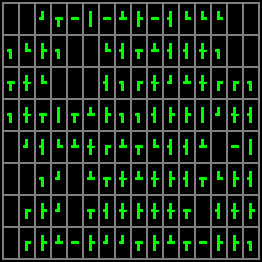
\includegraphics[scale=0.75]{SMT/pipe/shuffled.png}
\caption{Shuffled puzzle}
\end{figure}

\dots and solved:

\begin{figure}[H]
\label{fig:pipe_solved}
\centering
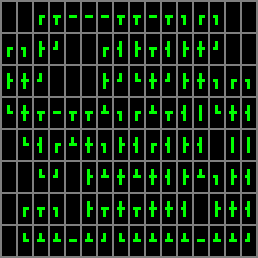
\includegraphics[scale=0.75]{SMT/pipe/solved.png}
\caption{Solved puzzle}
\end{figure}

Let's try to find a way to solve it.

\subsubsection{Generation}

First, we need to generate it.
Here is my quick idea on it.
Take 8*16 array of cells.
Each cell may contain some type of block.
There are joints between cells:

\pgfmathsetmacro\Width{16}
\pgfmathsetmacro\Height{8}
%\pgfmathsetmacro\Width{10}
%\pgfmathsetmacro\Height{5}
\pgfmathtruncatemacro\WidthMinusI{\Width - 1}
\pgfmathtruncatemacro\WidthMinusII{\Width - 2}
\pgfmathtruncatemacro\HeightMinusI{\Height - 1}
\pgfmathtruncatemacro\HeightMinusII{\Height - 2}
\pgfmathtruncatemacro\HeightPlusII{\Height + 2}
\pgfmathsetmacro\HeightPlusIi{\Height + 1.5}

% see also: http://www.texample.net/tikz/examples/euclid-algorithm/
\begin{center}
\begin{tikzpicture}[set style={{help lines}+=[dashed]},scale=0.7]

	\draw[style=help lines] (0,0) grid +(\Width,\Height);

	\foreach \c in {0,...,\WidthMinusI}
	{
		\foreach \r in {0,...,\HeightMinusII}
			\draw   [red,very thick,-] (\c+0.5,\r+0.75) -- (\c+0.5,\r+1.25);
		%\node[rotate=90] at (\c+0.5,\HeightPlusII) {\Large vjoints[\dots, \c] \normalsize};
		\node[rotate=90] at (\c+0.5,\HeightPlusII) {vjoints[\dots, \c]};
	}

	\foreach \r in {0,...,\HeightMinusI}
	{
		\foreach \c in {0,...,\WidthMinusII}
			\draw   [blue,very thick,-] (\c+0.75,\r+0.5) -- (\c+1.25,\r+0.5);
		\pgfmathtruncatemacro\hjointslabel{\HeightMinusI - \r}
		%\node at (-1.5,\r+0.5) {\large hjoints[\hjointslabel, \dots] \normalsize};
		\node at (-1.5,\r+0.5) {hjoints[\hjointslabel, \dots]};
	}

\end{tikzpicture}
\end{center}



Blue lines are horizontal joints, red lines are vertical joints.
We just set each joint to 0/false (absent) or 1/true (present), randomly.

Once set, it's now easy to find type for each cell.
There are:

\newcommand{\HeaderColor}{\cellcolor{blue!25}}
\begin{center}
\begin{longtable}{ | l | l | l | l | }
\hline
\HeaderColor joints & \HeaderColor our internal name & \HeaderColor angle & \HeaderColor symbol \\
\hline
0	&type 0		&	0$^{\circ}$	& (space)	\\
2	&type 2a	&	0$^{\circ}$	& \pmboxdrawuni{2503} \\ % ┃
2	&type 2a	&	90$^{\circ}$	& \pmboxdrawuni{2501} \\ % ━
2	&type 2b	&	0$^{\circ}$	& \pmboxdrawuni{250F} \\ % ┏
2	&type 2b	&	90$^{\circ}$	& \pmboxdrawuni{2513} \\ % ┓
2	&type 2b	&	180$^{\circ}$	& \pmboxdrawuni{251B} \\ % ┛
2	&type 2b	&	270$^{\circ}$	& \pmboxdrawuni{2517} \\ % ┗
3	&type 3		&	0$^{\circ}$	& \pmboxdrawuni{2523} \\ % ┣
3 	&type 3		&	90$^{\circ}$	& \pmboxdrawuni{2533} \\ % ┳
3	&type 3		&	180$^{\circ}$	& \pmboxdrawuni{252B} \\ % ┫
3	&type 3		&	270$^{\circ}$	& \pmboxdrawuni{253B} \\ % ┻
4	&type 4		&	0$^{\circ}$	& \pmboxdrawuni{254B} \\ % ╋
\hline
\end{longtable}
\end{center}

\textit{Dangling} joints can be preset at a first stage (i.e., cell with only one joint), but they are removed recursively,
these cells are transforming into empty cells.
Hence, at the end, all cells has at least two joints, and the whole plumbing system has no connections with outer
world---I hope this would make things clearer.

The C source code of generator is here: \url{https://github.com/dennis714/SAT_SMT_article/tree/master/SMT/pipe/generator}.
All horizontal joints are stored in the global array \textit{hjoints[]} and vertical in \textit{vjoints[]}.

The C program generates ANSI-colored output like it has been showed above (\ref{fig:pipe_shuffled}, \ref{fig:pipe_solved}) plus
an array of types, with no angle information about each cell:

\begin{lstlisting}[label=init_cells]
[
["0", "0", "2b", "3", "2a", "2a", "2a", "3", "3", "2a", "3", "2b", "2b", "2b", "0", "0"],
["2b", "2b", "3", "2b", "0", "0", "2b", "3", "3", "3", "3", "3", "4", "2b", "0", "0"],
["3", "4", "2b", "0", "0", "0", "3", "2b", "2b", "4", "2b", "3", "4", "2b", "2b", "2b"],
["2b", "4", "3", "2a", "3", "3", "3", "2b", "2b", "3", "3", "3", "2a", "2b", "4", "3"],
["0", "2b", "3", "2b", "3", "4", "2b", "3", "3", "2b", "3", "3", "3", "0", "2a", "2a"],
["0", "0", "2b", "2b", "0", "3", "3", "4", "3", "4", "3", "3", "3", "2b", "3", "3"],
["0", "2b", "3", "2b", "0", "3", "3", "4", "3", "4", "4", "3", "0", "3", "4", "3"],
["0", "2b", "3", "3", "2a", "3", "2b", "2b", "3", "3", "3", "3", "2a", "3", "3", "2b"],
]
\end{lstlisting}

\subsubsection{Solving}

First of all, we would think about 8*16 array of cells, where each has four bits:
``T'' (top),
``B'' (bottom),
``L'' (left),
``R'' (right).
Each bit represents half of joint.

% see also: http://www.texample.net/tikz/examples/euclid-algorithm/
\begin{center}
\begin{tikzpicture}[set style={{help lines}+=[dashed]},scale=0.7]

	\draw[style=help lines] (0,0) grid +(\Width,\Height);
	
	\foreach \c in {0,...,\WidthMinusI}
		%\node[rotate=90] at (\c+0.5,\HeightPlusIi) {\Large [\dots, \c] \normalsize};
		\node[rotate=90] at (\c+0.5,\HeightPlusIi) {[\dots, \c]};
	
	\foreach \r in {0,...,\HeightMinusI}
	{
		\pgfmathtruncatemacro\hlabel{\HeightMinusI - \r}
		%\node at (-1.5,\r+0.5) {\large [\hlabel, \dots] \normalsize};
		\node at (-1.5,\r+0.5) {[\hlabel, \dots]};
	
		\pgfmathsetmacro\Shift{0.325}
		\foreach \c in {0,...,\WidthMinusI}
		{
			\node at (\c+0.5,\r+0.5 + \Shift) {\footnotesize T \normalsize};
			\node at (\c+0.5,\r+0.5 - \Shift) {\footnotesize B \normalsize};
			\node at (\c+0.5 - \Shift,\r+0.5) {\footnotesize L \normalsize};
			\node at (\c+0.5 + \Shift,\r+0.5) {\footnotesize R \normalsize};
		}
	}

\end{tikzpicture}
\end{center}


Now we define arrays of each of four half-joints + angle information:

\begin{lstlisting}
HEIGHT=8
WIDTH=16

# if T/B/R/L is Bool instead of Int, Z3 solver will work faster
T=[[Bool('cell_%d_%d_top' % (r, c)) for c in range(WIDTH)] for r in range(HEIGHT)]
B=[[Bool('cell_%d_%d_bottom' % (r, c)) for c in range(WIDTH)] for r in range(HEIGHT)]
R=[[Bool('cell_%d_%d_right' % (r, c)) for c in range(WIDTH)] for r in range(HEIGHT)]
L=[[Bool('cell_%d_%d_left' % (r, c)) for c in range(WIDTH)] for r in range(HEIGHT)]
A=[[Int('cell_%d_%d_angle' % (r, c)) for c in range(WIDTH)] for r in range(HEIGHT)]
\end{lstlisting}

We know that if each of half-joints is present, corresponding half-joint must be also present, and vice versa.
We define this using these constraints:

\begin{lstlisting}
# shorthand variables for True and False:
t=True
f=False

# "top" of each cell must be equal to "bottom" of the cell above
# "bottom" of each cell must be equal to "top" of the cell below
# "left" of each cell must be equal to "right" of the cell at left
# "right" of each cell must be equal to "left" of the cell at right
for r in range(HEIGHT):
    for c in range(WIDTH):
        if r!=0:
            s.add(T[r][c]==B[r-1][c])
        if r!=HEIGHT-1:
            s.add(B[r][c]==T[r+1][c])
        if c!=0:
            s.add(L[r][c]==R[r][c-1])
        if c!=WIDTH-1:
            s.add(R[r][c]==L[r][c+1])

# "left" of each cell of first column shouldn't have any connection
# so is "right" of each cell of the last column
for r in range(HEIGHT):
    s.add(L[r][0]==f)
    s.add(R[r][WIDTH-1]==f)

# "top" of each cell of the first row shouldn't have any connection
# so is "bottom" of each cell of the last row
for c in range(WIDTH):
    s.add(T[0][c]==f)
    s.add(B[HEIGHT-1][c]==f)
\end{lstlisting}

Now we'll enumerate all cells in the initial array (\ref{init_cells}).
First two cells are empty there. And the third one has type ``2b''.
This is ``\pmboxdrawuni{250F}'' % ┏
and it can be oriented in 4 possible ways.
And if it has angle 0$^{\circ}$, bottom and right half-joints are present, others are absent.
If it has angle 90$^{\circ}$, it looks like 
``\pmboxdrawuni{2513}'', % ┓
and bottom and left half-joints are present, others are absent.

In plain English: ``if cell of this type has angle 0$^{\circ}$, these half-joints must be present \textbf{OR}
if it has angle 90$^{\circ}$, these half-joints must be present, \textbf{OR}, etc, etc.''

Likewise, we define all these rules for all types and all possible angles:

\begin{lstlisting}
for r in range(HEIGHT):
    for c in range(WIDTH):
        ty=cells_type[r][c]

        if ty=="0":
            s.add(A[r][c]==f)
            s.add(T[r][c]==f, B[r][c]==f, L[r][c]==f, R[r][c]==f)

        if ty=="2a":
            s.add(Or(And(A[r][c]==0, L[r][c]==f, R[r][c]==f, T[r][c]==t, B[r][c]==t),   # §\pmboxdrawuni{2503}§
                    And(A[r][c]==90, L[r][c]==t, R[r][c]==t, T[r][c]==f, B[r][c]==f)))  # §\pmboxdrawuni{2501}§

        if ty=="2b":
            s.add(Or(And(A[r][c]==0, L[r][c]==f, R[r][c]==t, T[r][c]==f, B[r][c]==t),   # §\pmboxdrawuni{250F}§
                    And(A[r][c]==90, L[r][c]==t, R[r][c]==f, T[r][c]==f, B[r][c]==t),   # §\pmboxdrawuni{2513}§
                    And(A[r][c]==180, L[r][c]==t, R[r][c]==f, T[r][c]==t, B[r][c]==f),  # §\pmboxdrawuni{251B}§
                    And(A[r][c]==270, L[r][c]==f, R[r][c]==t, T[r][c]==t, B[r][c]==f))) # §\pmboxdrawuni{2517}§
	
        if ty=="3":
            s.add(Or(And(A[r][c]==0, L[r][c]==f, R[r][c]==t, T[r][c]==t, B[r][c]==t),   # §\pmboxdrawuni{2523}§
                    And(A[r][c]==90, L[r][c]==t, R[r][c]==t, T[r][c]==f, B[r][c]==t),   # §\pmboxdrawuni{2533}§
                    And(A[r][c]==180, L[r][c]==t, R[r][c]==f, T[r][c]==t, B[r][c]==t),  # §\pmboxdrawuni{252B}§
                    And(A[r][c]==270, L[r][c]==t, R[r][c]==t, T[r][c]==t, B[r][c]==f))) # §\pmboxdrawuni{253B}§

        if ty=="4":
            s.add(A[r][c]==0)
            s.add(T[r][c]==t, B[r][c]==t, L[r][c]==t, R[r][c]==t) # §\pmboxdrawuni{254B}§
\end{lstlisting}

Full source code is here: \url{https://github.com/dennis714/SAT_SMT_article/blob/master/SMT/pipe/solver/solve_pipe_puzzle1.py}.

It produces this result (prints angle for each cell and (pseudo)graphical representation):

\begin{figure}[H]
\centering
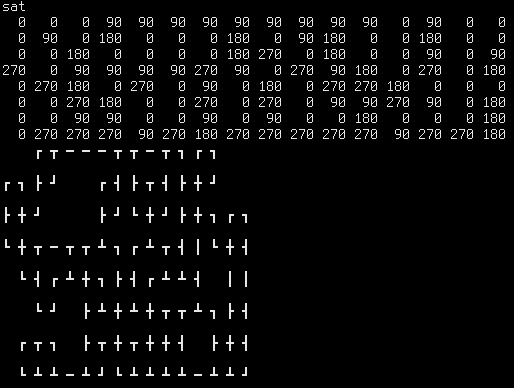
\includegraphics[scale=0.75]{SMT/pipe/solver/solver.png}
\caption{Solver script output}
\end{figure}

It worked $\approx 4$ seconds on my old and slow Intel Atom N455 1.66GHz.
Is it fast? I don't know, but again, what is really cool, we do not know about any mathematical background
of all this, we just defined cells, (half-)joints and defined relations between them.

Now the next question is, how many solutions are possible?
Using method described earlier (\ref{SMTEnumerate}), I've altered solver script
\footnote{\url{https://github.com/dennis714/SAT_SMT_article/blob/master/SMT/pipe/solver/solve_pipe_puzzle2.py}} and solver
said two solutions are possible.

Let's compare these two solutions using gvimdiff:

\begin{figure}[H]
\centering
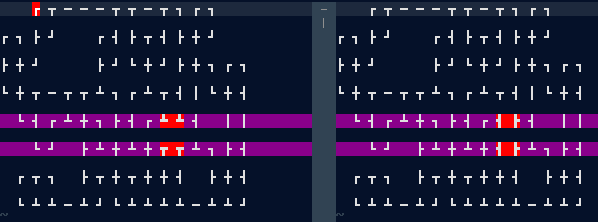
\includegraphics[scale=0.75]{SMT/pipe/solver/diff.png}
\caption{gvimdiff output (pardon my red cursor at left pane at left-top corner)}
\end{figure}

4 cells in the middle can be orientated differently.
Perhaps, other puzzles may produce different results.

P.S.
\textit{Half-joint} is defined as boolean type.
But in fact, the first version of the solver has been written using integer type for half-joints,
and 0 was used for False and 1 for True.
I did it so because I wanted to make source code tidier and narrower without using long words like ``False'' and ``True''.
And it worked, but slower. Perhaps, Z3 handles boolean data types faster? Better?
Anyway, I writing this to note that integer type can also be used instead of boolean, if needed.

